\documentclass[a4paper,10pt]{article}
\usepackage[utf8x]{inputenc}
\usepackage{amsmath}
\usepackage{graphicx}
\usepackage[english]{babel}
\usepackage{url}
\usepackage{epstopdf}
\usepackage{subfig}
\usepackage{graphicx}

\title{Procesamiento Avanzado de Imágenes\\IEE3784}
\author{\textbf{Tarea 01}\\Norman F. S\'aez\\nfsaez@uc.cl}
\date{\today}

\begin{document}
\maketitle
\section{Pregunta 1}
Utilizando los puntos dados en la tarea y el vector de nodos, se obtienen los siguientes gráficos:
\begin{figure}[ht!]
  \centering
  \subfloat[B-Splines]{\label{fig:img1}\includegraphics[width=0.50\textwidth]{img/img1.eps}}
  ~ 
  \subfloat[Bases]{\label{fig:img2}\includegraphics[width=0.50\textwidth]{img/img2.eps}}
  ~ 
  \caption{B-Splines y Bases}
  \label{fig:p1}
\end{figure}
La cantidad de sumas y de multiplicaciones son:
\begin{description}
\item[Sumas] 144
\item[Multiplicaciones] 60
\end{description} 
Para encontrar los graficos asi como las bases se utilizo la tecnica como sigue:
%Programe un software que construya B-splines cubicas no uniformes utilizando la recursion de Cox-de
%Boor vista en clase:
%Calcule el total de sumas y multiplicaciones necesarias para evaluar 100 puntos (por segmento) de
%la B-spline cubica (considere el caso mas favorable en terminos de operaciones e incluya las operaciones
%necesarias para construir las bases polinomiales).
%Para efectos del informe escrito, gra que en dos guras separadas la B-spline y las bases construidas
%con los siguientes puntos de control:
%y con el siguiente vector de nodos [1 3 4 7 7.5 10 20 25]

\end{document}
